\chapter{Økonomi} \label{Okonomi}
Formålet med dette afsnit er ud fra et økonomisk aspekt at vurdere, om en given teknologisk løsning er værd at implementere i praksis. I dette tilfælde gøres det ved at benytte omkostningsminimeringsanalyse. Den benyttes under antagelse af, at den sundhedsmæssige effekt er ens i den nuværende situation og i den fremtidige situation, hvor Ultralyds Robotarmen implementeres som en add-on løsning til det eksisterende ultralydsudstyr. \\
Der opstilles to scenarier. Scenarie 1 er den nuværende situation på en ultralydsscannings stue, mens scenarie 2 er den fremtidige situation på en stue med en Ultralyds Robotarm implementeret. I analysen ønskes det at klarlægge forskellene i de to scenarier i forhold til, hvilke ressource- og omkostningsforhold, der er i det enkelte scenarie. 

De økonomiske forskelle mellem de to situationer er opstillet i figur \ref{ModelOkonomi}. Figuren viser forskellene i, hvilke udgifter afdelingen vil have ved ultralydsscanninger af gravide med og uden brug af Ultralyds Robotarmen. Yderligere ses det, at der en række fællesudgifter ved begge situationer.  

\begin{figure}[H]\centering
	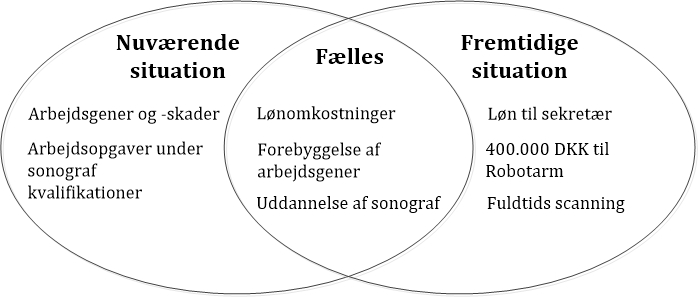
\includegraphics[width = 0.7\textwidth]{Figurer/ModelOkonomi}
	\caption{Økonomisk opdeling af udgifter i den nuværende og fremtidige situation, samt fællesnævnerer.}
	\label{ModelOkonomi}
\end{figure}

Belægget for dette afsnit er skabt på baggrund af interview med HEH, se Bilag 4. Her er deres arbejdsgange og arbejdsforhold blevet klarlagt. Se Kapitel \ref{Organisation} for yderligere beskrivelse heraf. Dermed er det vigtigt at pointere, at de praktiske forhold skal være sammenlignelige med HEH førend, der kan konkluderes tilsvarende for andre afdelinger.

Yderligere tager analysen udgangspunkt i, at CEO Søren Pallesen hos Robotic Ultrasound ApS forventer, at salgsprisen af Ultralyds Robotarmen med tilbehør bliver 400.000 DKK, se Bilag 6. \\
Scenarie 2 vil primært bygge på antagelser, da robotten ikke er færdigudviklet endnu. \\
Grundet at robotarmen er en add-on løsning til det eksisterende ultralydsudstyr, er priser på indkøb og vedligehold af ultralydsudstyret ikke medtaget. Det antages at disse priser er ens i begge scenarier. 

\section{Scenarie 1 - Den nuværende situation} \label{nuvaerende}
I dette scenarie fokuseres der på omkostnings- og ressourceforbruget for at holde en ultralydsscannings stue i drift fem dage om ugen. I den nuværende situation scanner en sonograf fire dage om ugen, mens sonografen den femte dag varetager en række arbejdsopgaver, som sonografen er overkvalificeret til. Dette skyldes, at det ønskes at aflaste sonograferne i deres arbejdsforhold og dermed mindske mængden af arbejdsgener og potentielle arbejdsskader. Denne organisering af arbejdet er et valg foretaget af afdelingens ledelse, se Bilag 4. \\ 
Omkostningerne i den nuværende situation kan opdeles i følgende punkter:

\begin{itemize}
\item Lønomkostninger til 1,2 sonograf
\item Arbejdsgener 
\item Udgifter til forebyggelse
\item Uddannelse af sonografer
\end{itemize}
Lønomkostninger er, i dette scenarie, givet ved 1,2 sonograf. 1,2 sonograf er estimeret på baggrund af, at det er nødvendigt at have en sonograf plus 1/5 af en anden sonografs arbejdstid for at have stuen bemandet fem dage om ugen. En sonograf med 2 års erfaring og kvalifikationstillæg er på løntrin 6, hvilket giver en månedsløn på 26.967 DKK, se Bilag 4. På årsbasis giver det en årsløn på 323.604 DKK. Lønudgifter er dermed beregnet til:
\begin{equation}
323.604 \text{ DKK}\cdot1,2 = 388.325 \text{ DKK}
\end{equation}
Det ses også, at i den nuværende organisering af arbejdsgangen er der taget hensyn til, at scanning af gravide er et belastende arbejde. Dette viser sig gennem en række omkostninger til forebyggelse af arbejdsskader og -gener. Det er en økonomisk udgift, at en sonograf ikke kan scanne fuldtid og dermed bliver nødsaget til at påtage sig opgaver, sonografen er overkvalificeret til, se Bilag 4. Det vil være omkostningsmæssigt billigere, hvis opgaverne bliver varetaget af en person, hvis kvalifikationsniveau passer dertil. Denne person vil typisk modtage en lavere løn end sonografen og dermed føre til en besparelse.

Samtidig findes udgifter til skadeforebyggelse såsom ergonomiske stole, elastik-træning, massage i arbejdstiden og wellness-konsulenter, der står til rådighed for at give sonograferne råd og vejledning om bedre arbejdsstillinger og -forhold, se Bilag 4. Det har ikke været muligt at finde tilstrækkeligt oplysninger om udgifterne hertil, dermed er disse ikke medtaget i beregningerne. 

Yderligere er der omkostninger forbundet med uddannelse af sonografer. Uddannelse af en sonograf er estimeret til at koste 108.000 DKK, se Bilag 4. Uddannelsen foregår som mesterlære over en 16 ugers periode. I denne periode er den nye sonograf altid under vejledning af mesteren. Dermed er der dobbeltbemanding på hver scanning. Således antages det, at prisen på uddannelsen er givet ved lønomkostninger til den ekstra mand, i form af mesteren, i de 16 uger:
\begin{equation}
27.000 \text{ DKK}\cdot4 \text{ måneder} = 108.000 \text{ DKK}
\end{equation}
Der er også forbundet omkostninger ved, at sonografen først antages at kunne foretage alle typer scanninger på egen hånd efter to år, se Bilag 4. Dermed kan der være forlængede scanningstider for den nye sonograf, såfremt vedkommende støder på ukendte scenarier og dermed bliver nødsaget til at opsøge hjælp fra mere erfarne sonografer.

Fra et regionsperspektiv er der ikke direkte omkostninger forbundet med, at en sonograf pådrager sig en arbejdsskade. Ses situationen fra et samfundsperspektiv, vil det kunne føre til afledte omkostninger i form af, at personen bliver nedslidt af arbejdet og tvunget tidligere på pension. Denne persons samlede livsløn vil være lavere end en sonograf, der har været på arbejdsmarkedet et fuldt arbejdsliv. Dette fører til, at personen relativt vil være en økonomisk udgift fremfor at bidrage økonomisk til samfundet. 

Hvor stort et problem arbejdsgener er økonomisk, er svært at måle. En arbejdsgene viser sig som en smerte, men det er svært at angive smerteværdien i kroner og øre. Yderligere er det svært
at svare på, om smerten fremkommer af scanningsarbejdet eller af en fritidsinteresse, se Bilag 4. Dette gør, at arbejdsgener viser sig som afledte omkostninger. Det har ikke været muligt at finde konkrete tal på arbejdsgener og sygedage blandt sonografer, hvor årsagen til lidelsen kan føres tilbage til scanningsarbejdet.  

\section{Scenarie 2 - Den fremtidige situation} \label{fremtidige}
I dette scenarie fokuseres der på de ressourcer, der vil komme i spil ved implementering af en Ultralyds Robotarm som en add-on løsning til eksisterende ultralydsudstyr. Der tages ligeledes udgangspunkt i omkostnings- og ressourceforbruget for at holde en ultralydsscannings stue i drift fem dage om ugen. I dette afsnit vil der blive trukket paralleller til scenarie 1 for at tydeliggøre, hvor omkostnings forskellene er. \\
Omkostningerne i den fremtidige situation er givet ved følgende punkter:
\begin{itemize}
\item 400.000 DKK til Ultralyds Robotarm
\item Udgifter til forebyggelse
\item Regionens ansvar for personale og arbejdsmiljø
\item Lønomkostninger
\item Uddannelse af sonografer til brug af robotarm
\end{itemize}
Etableringsomkostninger til Ultralyds Robotarmen er estimeret til at være 400.000 DKK, se Bilag 6.
For de fleste institutioner vil en sådan udgift være et stort udlæg, derfor er det mere relevant at fordele omkostninger over den årrække, som indkøberne afskriver teknologien over. Afskrivningsperioden er på ti år, da det er estimeret, at udstyret er forældet efter denne periode. Eksisterende ultralydsudstyr afskrives ligeledes over ti år, se Bilag 4.

Fordeles etableringsomkostningerne efter annuitetsmetoden med en forrentningsfaktor på 0,9\% \cite{Inflationsrate}, se Forkortelser og formler, formel 1. Forrentningsfaktoren er estimeres til at være inflationsraten i Danmark i 2016. Årligt giver dette en omkostning på 42.007 DKK:

\begin{equation}
\left(\frac{(1+0,009)^{10}\cdot0,009}{(1+0,009)^{10}-1}\right)\cdot400.000 \text{ DKK}=42.007 \text{ DKK}
\end{equation}

I dette scenarie antages det, at der ikke vil opstå arbejdsgener grundet scanningsarbejdet ved brug af Ultralyds Robotarmen, se Kapitel \ref{aktoerer_organisation}. 

Udgifterne til forebyggelse vil stadig være til stede for afdelingen, da ergonomiske stole, massage og elastik-træning stadig vil være en forbedrende faktor for sonografers arbejdssforhold. Robotarmen kan bruges til cirka 70-80\% af scanningerne, hvilket medfører, at sonografer stadig vil blive belastet som i den nuværende situation i cirka 20-30\% af scanningerne, se Bilag 12, 28.04.2016. Dermed kan afdelingen ikke se bort fra udgiften til sundhedsforebyggelse og -fremmende løsninger i fremtiden.  

I scenarie 2 vil regionen have udgiften til robotarmen på 400.000 DKK som en meromkostning, hvilket vil være et stort udlæg, hvis der udelukkende ses på beløbene. Samtidig har regionen også et ansvar for dens personale og arbejdsmiljø, herunder sikkerhed og sundhed. \\
Ansvaret gør, at regionen ikke udelukkende kan fokusere på direkte udgifter, men også skal medtage andre aspekter, når en ny teknologi skal implementeres for at forbedre arbejdsforhold for personalet. Der ligger en forventning fra samfundet om, at regionen påtager sig ansvaret for personalet og arbejdsmiljøet. Regionen bidrager på den måde til, at personalet kan blive i deres job i flere år \cite{Arbejdsmiljo}\cite{RegionAnsvar}. 

Det sidste forhold, der er medtaget i denne analyse, er forskellene i lønomkostninger. I scenarie 1 skal der 1,2 sonograf til for at bemande en stue fem dage om ugen. I scenarie 2 skal der 1 sonograf til, da det antages, at en sonograf nu kan scanne på fuldtid, se Bilag 4. Dette giver følgende lønomkostninger for én sonograf på én stue på årsbasis:
\begin{equation}
323.604 \text{ DKK}\cdot1 = 323.604 \text{ DKK/stue/år}
\end{equation}
De arbejdsopgaver, som sonografen ikke har tid til at varetage i scenarie 2, skal udføres af en anden, eksempelvis en lægesekretær. En lægesekretærs bruttotimeløn på løntrin 24 er givet ved 159,84 DKK \cite{Lontabel}. En standard arbejdsdag er 7,4 timer \cite{Arbejdstid}. Lønudgifterne til sekretæren for én dag om ugen i et arbejdsår, kan således beregnes:
\begin{equation}
159,84 \text{ DKK/time} \cdot 7,4 \text{ timer} \cdot 52 \text{ uger} = 61.516 \text{ DKK/år}
\end{equation}
De samlede lønomkostninger, for én sonograf og én lægesekretær, til at holde en stue i drift på årsbasis, hvor de samme arbejdsopgaver, der blev udført i scenarie 1 er medtaget, er beregnet til:
\begin{equation}
323.604 \text{ DKK/stue/år} + 61.516 \text{ DKK/år} = 385.120 \text{DKK/stue/år}
\end{equation}
Behovet for færre sonografer til bemanding af én stue vil føre til, at færre sonografer skal uddannes. Dette vil give en økonomisk besparrelse for regionen, da udgifterne til uddannelse af sonografer vil blive nedsat. Der vil ved implementeringen af robotarmen komme en meromkostning til uddannelse i brugen der af. Dette aspekt er ikke medtaget i beregningerne. 

\section{Perspektivering til RMV}
Set fra et økonomisk perspektiv er omkostningerne til at holde en stue i drift på RMV sammenlignelige med de beskrevne for HEH, se Bilag 4 og Bilag 5. En markant forskel på RMV og HEH er indretningen af stuerne, hvor det vil blive nødvendigt at ommøblere for at få plads til Ultralyds Robotarmen. 
Denne omkostnings- og ressourceanalyse er mulig at overføre til lignende afdelinger på andre hospitaler i Danmark. Der vil være variationer i udgifter til uddannelse af sonografer, alt efter afdelingens organisering. Ligeledes vil afdelingens geografisk placering give variationer i lønudgifterne. 

\section{Delkonklusion}
Gennemgangen af omkostnings- og ressourceforskelle mellem scenarie 1 og scenarie 2 viser, at der er en række fordele ved scenarie 1 såvel som scenarie 2. Den afgørende faktor er dermed op til den potentielle køber at afgøre. De største forskelle er mængden af arbejdsskader og -gener, lønomkostninger og udgift til anskaffelse af Ultralyds Robotarmen. Sonografuddannelsen vil være en udgift i begge scenarier og bidrager på kort sigt ikke til en betydende forskel. 

Ses der udelukkende på de direkte omkostninger vil scenarie 1 være den løsning med færrest
omkostninger. Dette skyldes, at scenarie 2 er dyrere i direkte omkostninger, da robotarmen er en
add-on. Besparelsen på 3.205 DKK mellem scenarie 1 og scenarie 2 i årlige lønomkostninger dækker ikke udgiften til robotarmens årlige afskrivning på 42.007 DKK. \\
Medtages de indirekte og afledte omkostninger, vil scenarie 2 give mulighed for besparelser i forhold til arbejdsskader og -gener, samt en bedre fordeling af opgaver i forhold til personalets kvalifikationsniveau. Dette kan opveje for udgifterne til robotarmen, men vil være afhængig af den enkelte hospitalsafdeling. Scenarie 2 giver mulighed for længere tid på arbejdsmarkedet, hvilket giver færre omkostninger for samfundet.

